\documentclass{article}

\usepackage{graphicx}
\usepackage{tikz}
\usepackage{tikzsymbols}
\usetikzlibrary{calc,patterns,shapes.geometric}
\pagestyle{empty}
\usepackage[margin=0pt]{geometry}
\geometry{papersize={14in,12in}}

\def\centerarc[#1](#2)(#3:#4:#5){\draw[#1] ($(#2)+({#5*cos(#3)},{#5*sin(#3)})$) arc (#3:#4:#5);}

\begin{document}
	\begin{figure}
		\centering
		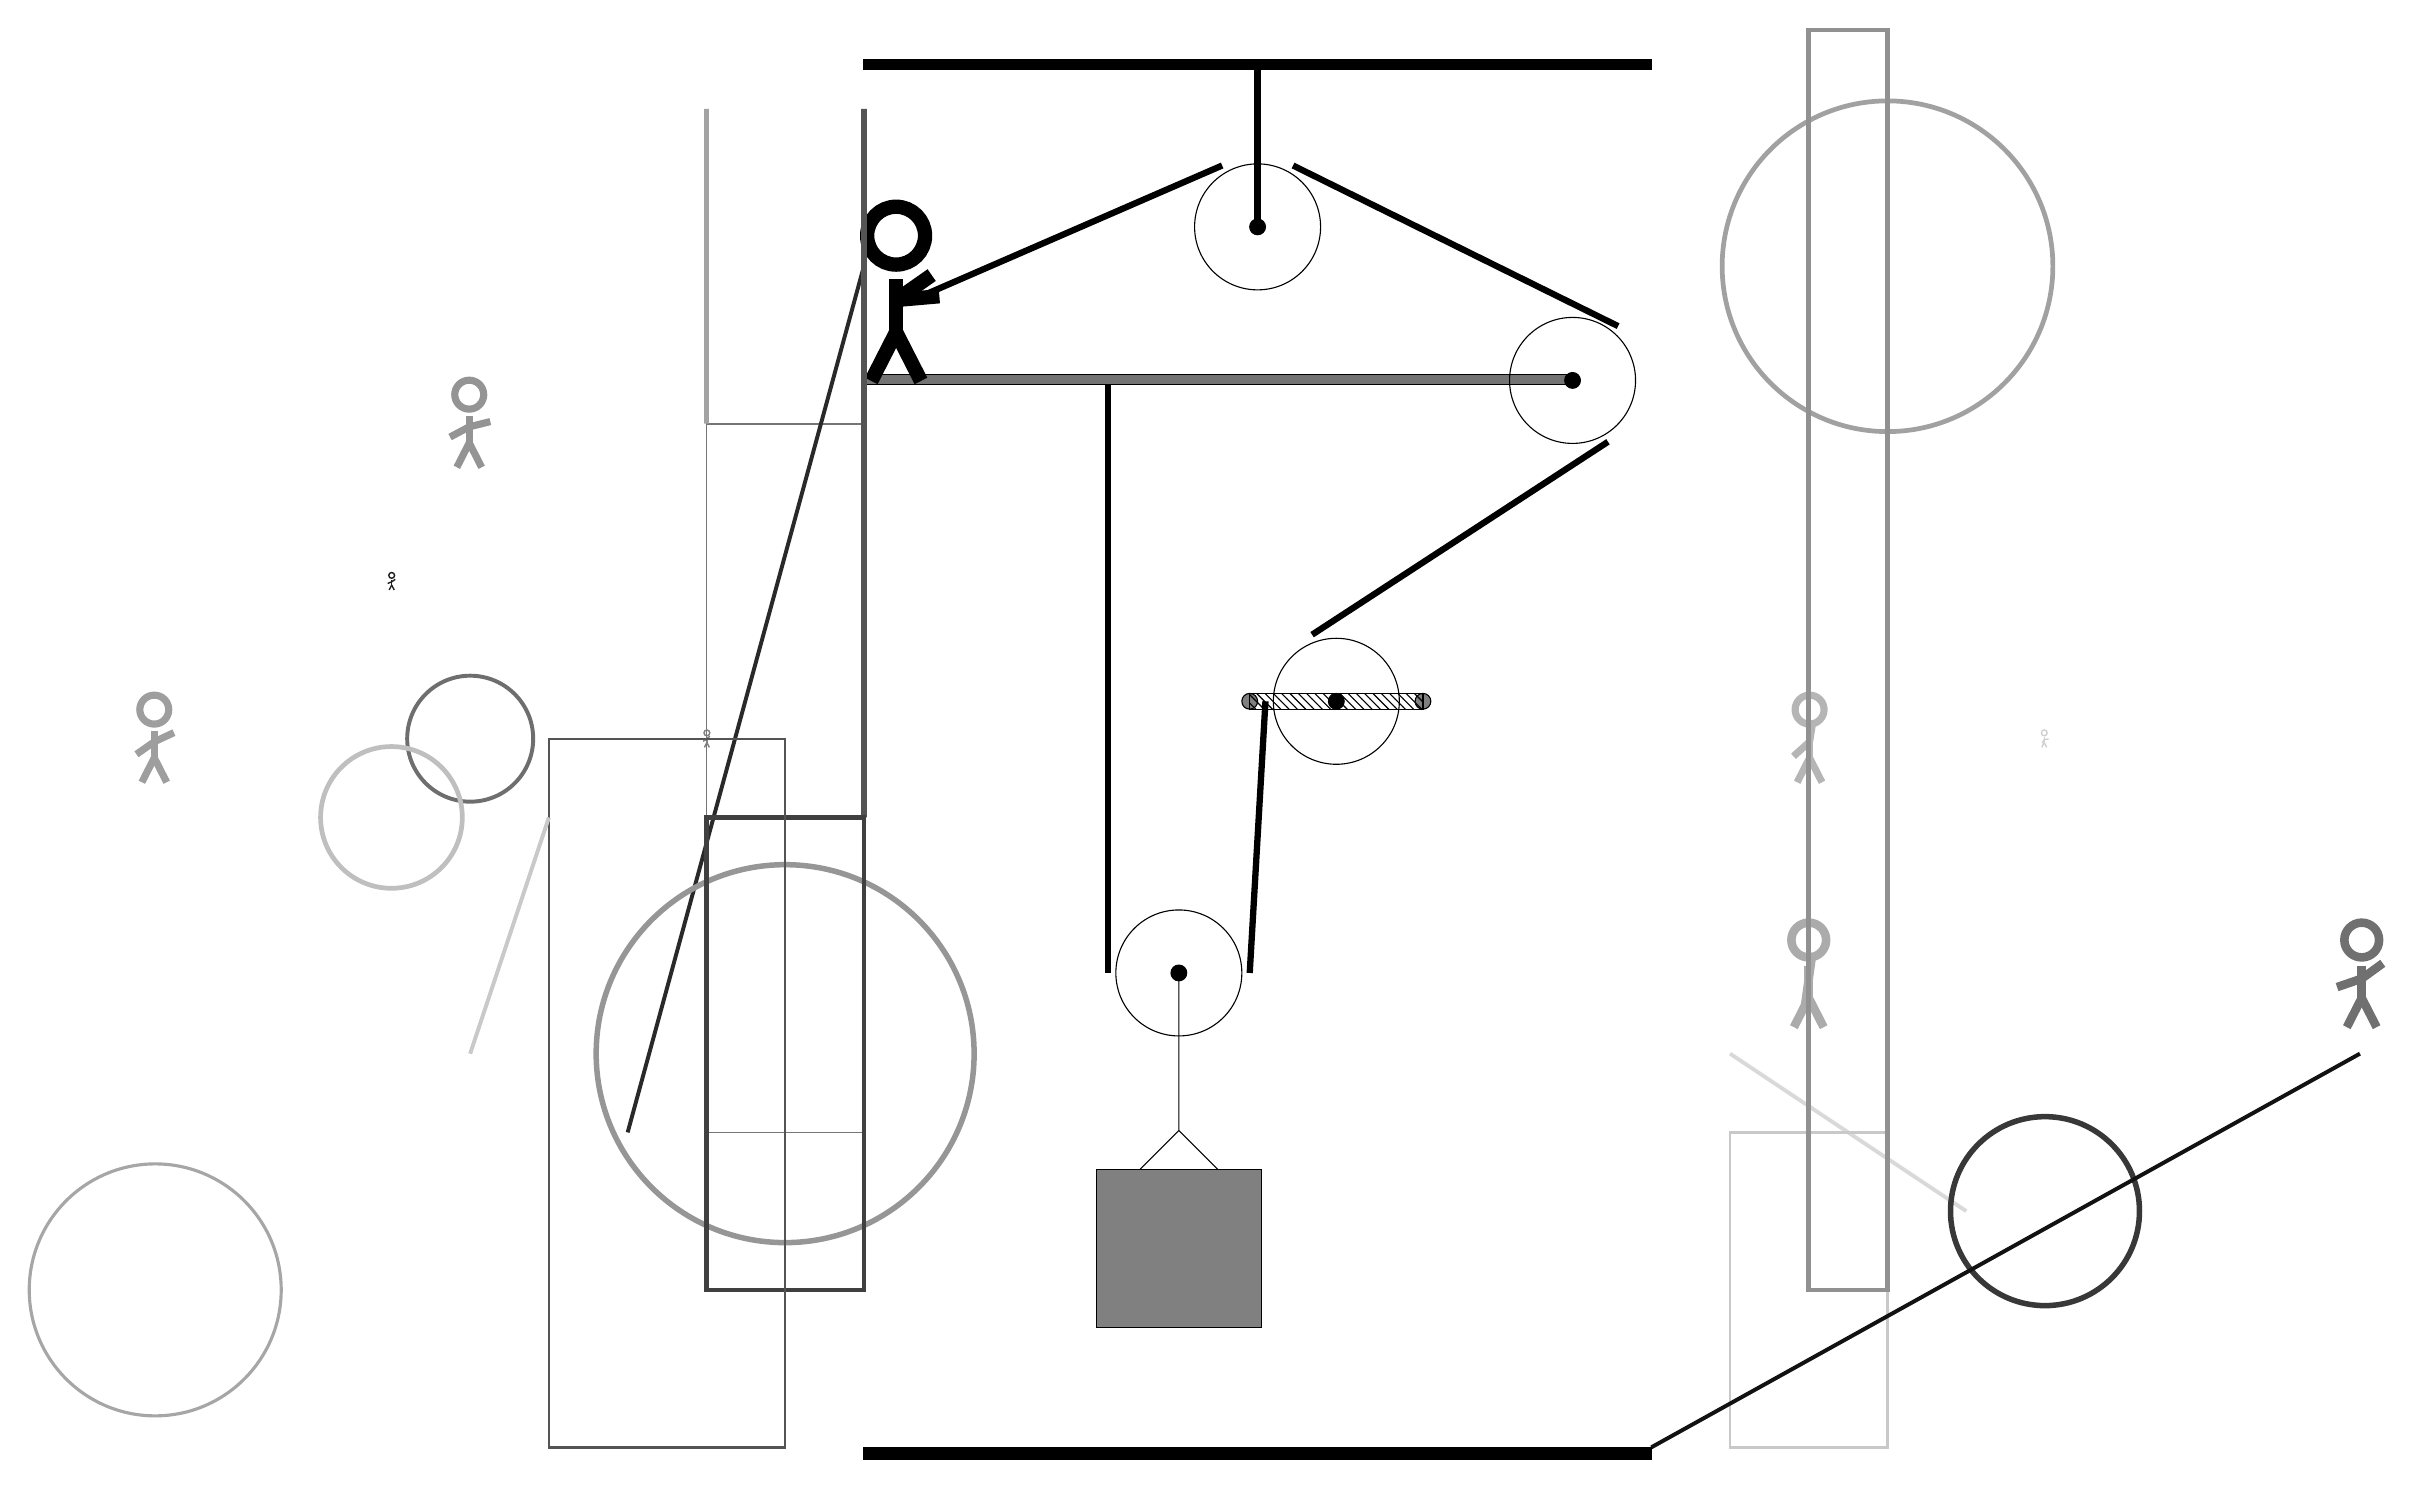
\begin{tikzpicture}
			%%%%% START %%%%%
			
			\draw[fill=black] (-2, 15.5) rectangle (8, 15.625);
			
			\draw[fill=black!55] (-2, 11.5) rectangle (7, 11.625);
			
			\draw (2, 4.025) circle (0.8);
			\draw[fill=black] (2, 4.025) circle (0.1);
			
			\draw (7, 11.55) circle (0.8);
			\draw[fill=black] (7, 11.55) circle (0.1);
			
			\draw[fill=white](4, 7.475) circle (0.8);
			\draw[fill=black] (4, 7.475) circle (0.1);
			\draw[fill=black!50] (2.9, 7.475) circle (0.1);
			\draw[fill=black!50] (5.1, 7.475) circle (0.1);
			\draw[pattern=north west lines, pattern color=black] (2.9, 7.575) rectangle (5.1, 7.375);
			
			\draw (3, 13.5) circle (0.8);
			\draw[fill=black] (3, 13.5) circle (0.1);
			\draw[line width=0.8mm] (3, 13.5) -- (3, 15.5);
			
			\draw (2, 4.025) -- (2, 2.025) -- (1.5, 1.525) -- (2.5, 1.525) -- (2, 2.025);
			\draw[fill=black!50] (0.95, 1.525) rectangle (3.05, -0.475);
			
			\draw[line width=0.8mm] (1.1, 11.5) -- (1.1, 4.025);
			\centerarc[line width=0.8mm](2, 4.025)(180:360:0.9);
			\draw[line width=0.8mm](2.9, 4.025) -- (3.1, 7.475);
			\centerarc[line width=0.8mm](4, 7.475)(110:180:0.9);
			\draw[line width=0.8mm](3.6922, 8.3207) -- (7.45, 10.7706);
			\centerarc[line width=0.8mm](7, 11.55)(-60:50:0.9);
			\draw[line width=0.8mm](7.5785, 12.2394) -- (3.45, 14.2794);
			\centerarc[line width=0.8mm](3, 13.5)(60:120:0.9);
			\draw[line width=0.8mm](2.55, 14.2794) -- (-1.2, 12.65);
			
			\node at (-1.5, 12.65) {\Strichmaxerl[10][-175][35]};
			
			\draw[line width=0.2mm, color=black!54] (-2, 2) rectangle (-4, 11);
			
			\node[line width=0.3mm, color=black!50] at (-4, 7) {\Strichmaxerl[1][27][48]};
			\node[line width=0.4mm, color=black!56] at (17, 4) {\Strichmaxerl[6][19][36]};
			\draw [line width=0.6mm, color=black!37](11, 13) circle (2.1);
			\draw[line width=0.5mm, color=black!84](-2, 13) -- (-5, 2);
			\draw [line width=0.5mm, color=black!57](-7, 7) circle (0.8);
			\node[line width=0.4mm, color=black!42] at (-7, 11) {\Strichmaxerl[5][28][14]};
			\draw[line width=0.7mm, color=black!67] (-2, 6) rectangle (-2, 15);
			\draw [line width=0.7mm, color=black!41](-3, 3) circle (2.4);
			\draw[line width=0.5mm, color=black!15](9, 3) -- (12, 1);
			
			\draw [line width=0.7mm, color=black!78](13, 1) circle (1.2);
			
			\draw[line width=0.6mm, color=black!75] (-4, 0) rectangle (-2, 6);
			\draw[line width=0.3mm, color=black!67] (-3, 7) rectangle (-6, -2);
			
			\draw [line width=0.4mm, color=black!35](-11, 0) circle (1.6);
			\node[line width=0.3mm, color=black!29] at (10, 7) {\Strichmaxerl[5][42][81]};
			\draw[line width=0.3mm, color=black!21] (9, -2) rectangle (11, 2);
			
			\node[line width=0.6mm, color=black!18] at (13, 7) {\Strichmaxerl[1][62][2]};
			
			\node[line width=0.5mm, color=black!33] at (10, 4) {\Strichmaxerl[6][82][82]};
			\draw [line width=0.6mm, color=black!25](-8, 6) circle (0.9);
			\draw[line width=0.7mm, color=black!36] (-4, 15) rectangle (-4, 11);
			\draw[line width=0.5mm, color=black!21](-7, 3) -- (-6, 6);
			
			\node[line width=0.5mm, color=black!88] at (-8, 9) {\Strichmaxerl[1][22][35]};
			
			\node[line width=0.5mm, color=black!38] at (-11, 7) {\Strichmaxerl[5][35][25]};
			\draw[line width=0.5mm, color=black!93](8, -2) -- (17, 3);
			\draw[line width=0.6mm, color=black!43] (10, 0) rectangle (11, 16);
			
			\draw[fill=black] (-2, -2) rectangle (8, -2.15);
			
			%%%%% END %%%%%
		\end{tikzpicture}
	\end{figure}	
\end{document}